\chapter{يولد وينمو ويموت}\label{ch:g2:born-grow-die}

في الربيع تكتسي شجرة الكرز عند البوابة بالزهر؛ وتحتها ترضع قطة
هريراتها المولودة حديثًا؛ ويعرض الجد صورة له وهو في مثل سنّك ---
صغيرًا، مفلوج الأسنان، ومولعًا بالكرز منذ ذلك الحين. كل \omterm{def:g1:living-or-not:living}{كائن حي}
يسلك الطريق نفسه: يبدأ، وينمو، وينتهي يومًا ما. ويسمى هذا الطريق
\omterm{def:g2:born-grow-die:cycle}{دورة الحياة}.

\section{مراحل الحياة}

\begin{definition}[دورة الحياة]\label{def:g2:born-grow-die:cycle}
\emph{دورة حياة}\index{دورة الحياة} \omterm{def:g1:living-or-not:living}{الكائن الحي} هي سلسلة
\emph{المراحل}\index{مرحلة} التي تمر بها حياته:
\begin{enumerate}
  \item \emph{يولد}\index{ولادة} --- وهذه البداية؛
  \item ويكون \emph{صغيرًا}\index{صغير} --- فينمو ويتغير بسرعة؛
  \item ثم يصير \emph{بالغًا}\index{بالغ} --- تام النمو؛ والبالغون
        يمكن أن يكون لهم صغار؛
  \item ثم \emph{يشيخ}\index{شيخوخة}، وفي النهاية
        \emph{يموت}\index{موت}.
\end{enumerate}
\end{definition}

\begin{example}[ثلاث حيوات وطريق واحد]\label{ex:g2:born-grow-die:three}
يولد هرّ صغير، فيلعب وينمو حتى يصير قطة قد تكون لها هريرات، ثم
تشيخ. وتنبت بذرة كرز، وتطول الشجرة الصغيرة سنوات، ثم تصنع الشجرة
البالغة الزهر والكرز، وبعد عشرات السنين تموت. وأنت كذلك: رضيع، ثم
طفل، ثم كبير يومًا ما. الهر الصغير، وشجرة الكرز، والطفل --- \omterm{def:g2:born-grow-die:cycle}{المراحل}
الأربع نفسها.
\end{example}

\begin{omfigure}
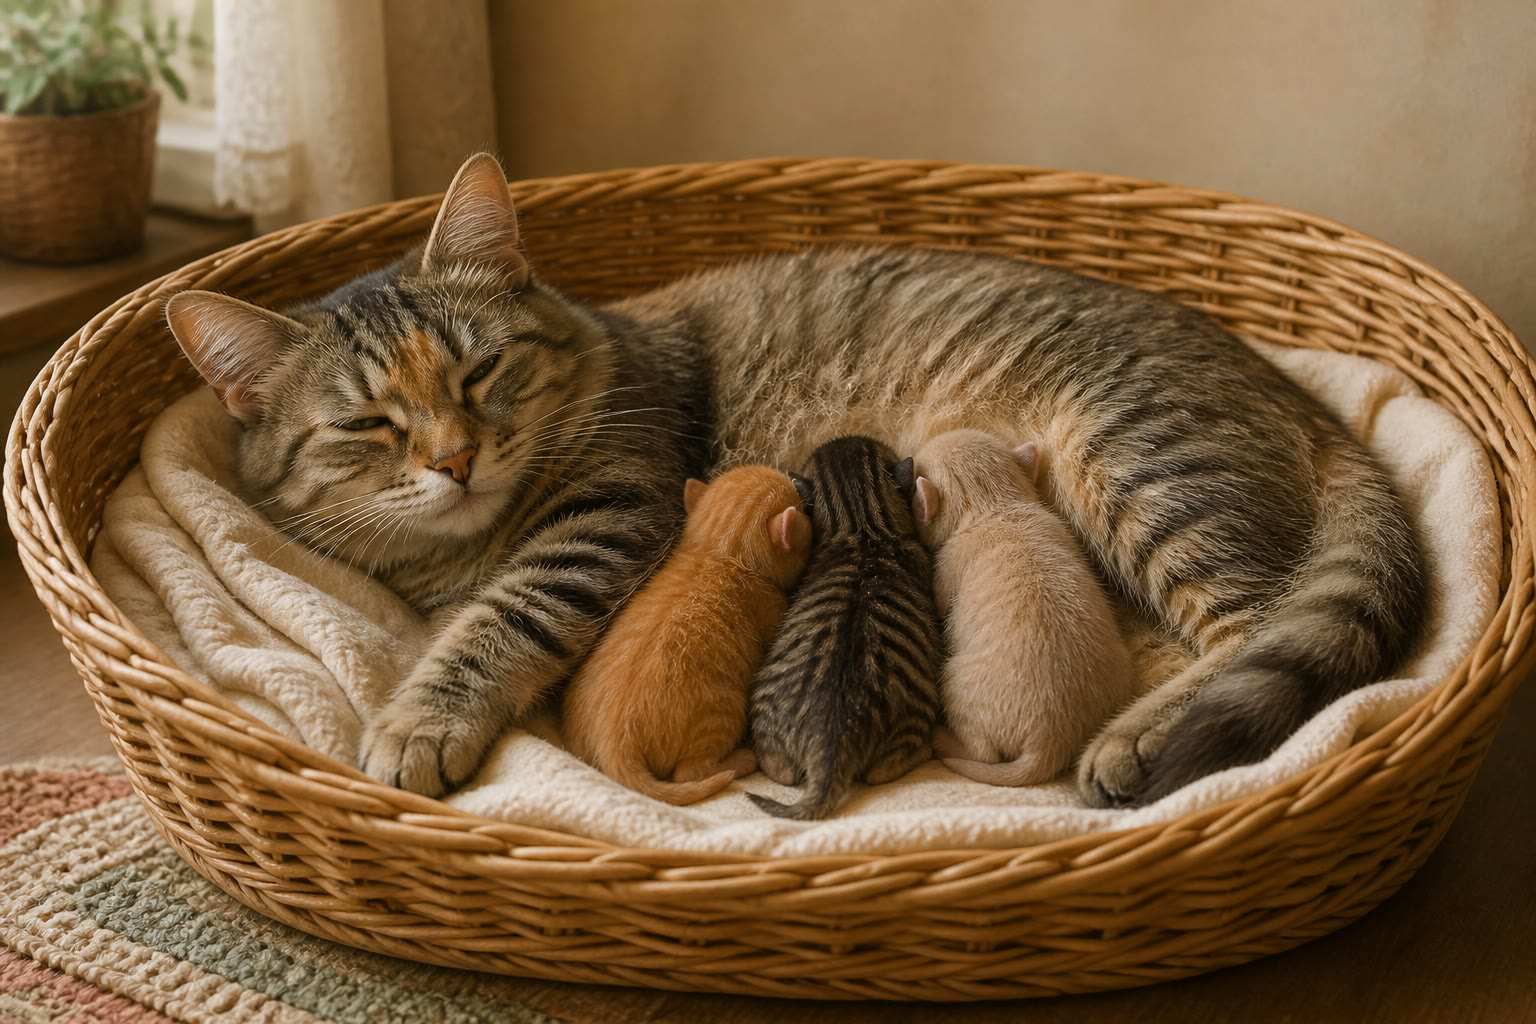
\includegraphics[width=0.62\linewidth]{images/book1/ai/g2-cycle-kittens.jpg}

{\small بداية ثلاث دورات حياة في وقت واحد: هريرات حديثة \omterm{def:g2:born-grow-die:cycle}{الولادة}
عند حليب أمها.}
\end{omfigure}

\begin{omfigure}
\begin{tikzpicture}[scale=0.92]
  \foreach \x/\txt in {0/{ولادة},3.1/{صغر},6.2/{بلوغ},9.3/{شيخوخة}} {
    \draw[thick, omDef, fill=omDef!7, rounded corners=5pt]
      (\x,0) rectangle ({\x+2.4},1.2);
    \node[font=\small\bfseries, text height=1.6ex, text depth=0.4ex]
      at ({\x+1.2},0.6) {\txt};
  }
  \draw[->, thick, omMeth] (2.4,0.6) -- (3.1,0.6);
  \draw[->, thick, omMeth] (5.5,0.6) -- (6.2,0.6);
  \draw[->, thick, omMeth] (8.6,0.6) -- (9.3,0.6);
  % new generation arrow
  \draw[->, thick, omProp] (7.4,1.2) .. controls (7.4,2.3) and (1.2,2.3)
    .. (1.2,1.25);
  \node[font=\small, omProp] at (4.3,2.35) {للبالغين صغار: تبدأ دورة جديدة};
\end{tikzpicture}

{\small مراحل الحياة --- والسهم الذي يبدأ الطريق من جديد مع الجيل
التالي.}
\end{omfigure}

\begin{remark}[لماذا سميت دورة]\label{rem:g2:born-grow-die:wheel}
كل حياة مفردة تجري من \omterm{def:g2:born-grow-die:cycle}{الولادة} إلى الموت، كطريق له طرفان. لكن قبل
النهاية يكون للبالغين صغار، وأولئك الصغار يبدؤون الطريق من جديد.
وإذا نظرنا عبر أجيال كثيرة، دارت الحياة كالعجلة --- ولهذا نقول
\emph{دورة} الحياة.
\end{remark}

\section{النمو والتغير}

\begin{proposition}[الكبر أكثر من ازدياد الحجم]\label{prop:g2:born-grow-die:change}
في أثناء نموه \emph{يتغير} \omterm{def:g1:living-or-not:living}{الكائن الحي} الصغير أيضًا: فالرضيع تنبت
له أسنان، ثم تسقط، ثم تنبت أقوى منها؛ وزغب الكتكوت الأصفر يصير
ريشًا حقيقيًّا؛ \omterm{def:g1:plants-around-us:parts}{وساق} الشجرة الصغيرة الطرية الخضراء تصير خشبًا صلبًا.
فالنمو ازدياد في الحجم \emph{وصيرورة} إلى شيء مختلف.
\end{proposition}
\admitted

\begin{example}[اختبار الصورة]\label{ex:g2:born-grow-die:photo}
في صور الجد القديمة يمكنك تتبع شخص واحد عبر كل \omterm{def:g2:born-grow-die:cycle}{مرحلة}: رضيع، ثم
تلميذ، ثم شاب، ثم أب، ثم جدّ. الشخص نفسه، والجسم يتغير. والصور
آلات زمن صغيرة لمشاهدة \omterm{def:g2:born-grow-die:cycle}{دورة حياة}.
\end{example}

\begin{method}[ترتيب مراحل الحياة]\label{met:g2:born-grow-die:order}
إذا أُعطيت صورًا مختلطة لحياة \omterm{def:g1:living-or-not:living}{كائن حي}:
\begin{enumerate}
  \item جد صورة \omterm{def:g2:born-grow-die:cycle}{الولادة} --- بيضة، أو بذرة، أو مولودًا حديثًا؛
  \item وجد \omterm{def:g2:born-grow-die:cycle}{البالغ} --- تام النمو، قادرًا على أن يكون له صغار؛
  \item وضع الصغار بينهما، من الأصغر إلى الأكبر؛
  \item وراجع صفّك: أتؤدي كل صورة إلى التي بعدها؟
\end{enumerate}
\end{method}

\section{كل حياة تنتهي --- والحياة تمضي}

\begin{proposition}[مدة الحياة]\label{prop:g2:born-grow-die:lifespan}
تعيش الكائنات الحية المختلفة مددًا مختلفة --- وهي \emph{مدة
الحياة}\index{مدة الحياة}. فالفراشة قد تعيش أسابيع قليلة؛ والقطة
والكلب من عشر سنوات إلى عشرين؛ والإنسان أكثر من ثمانين سنة في
الغالب؛ وبعض الأشجار مئات السنين. وطالت المدة أم قصرت، فلكل حياة
نهاية.
\end{proposition}
\admitted

\begin{example}[شجرة التفاح العجوز]\label{ex:g2:born-grow-die:oldtree}
شجرة التفاح العجوز المنحنية في آخر الحديقة تعطي تفاحًا أقل كل سنة
--- إنها في شيخوختها. لكن في تفاحها بذورًا، وبذرة واحدة تُزرع هي
شجرة تفاح صغيرة تبدأ الطريق. وحين تموت الشجرة العجوز لن تنقرض
أشجار التفاح: فصغارها تكمل المسير.
\end{example}

\begin{remark}[الحديث عن الموت]\label{rem:g2:born-grow-die:death}
الموت جزء من كل \omterm{def:g2:born-grow-die:cycle}{دورة حياة}، ولا بأس أن نحزن له --- والناس يحزنون،
وخاصة على \omterm{def:g1:animals-around-us:animal}{الحيوانات} الأليفة وعلى من نحب. ويضيف \omterm{def:g1:living-or-not:living}{علم الأحياء} عزاء
واحدًا: لأن للبالغين صغارًا قبل أن يموتوا، فالحياة نفسها تستمر،
دورة بعد دورة.
\end{remark}

\section{تمارين}

\begin{exercise}[$\star$]\label{exo:g2:born-grow-die:1}
سمِّ مراحل \omterm{def:g2:born-grow-die:cycle}{دورة الحياة} الأربع، مرتبةً.
\end{exercise}

\begin{exercise}[$\star$]\label{exo:g2:born-grow-die:2}
في أي \omterm{def:g2:born-grow-die:cycle}{مرحلة} يمكن أن يكون \omterm{def:g1:living-or-not:living}{للكائن الحي} صغار؟
\end{exercise}

\begin{exercise}[$\star$]\label{exo:g2:born-grow-die:3}
رتّب من الأكبر سنًّا إلى الأصغر: تلميذ، ورضيع، وجدّة، وأمّ.
\end{exercise}

\begin{exercise}[$\star$]\label{exo:g2:born-grow-die:4}
اذكر \omterm{def:g2:born-grow-die:cycle}{دورة حياة} شجرة الكرز في \cref{ex:g2:born-grow-die:three}،
مرحلةً \omterm{def:g2:born-grow-die:cycle}{مرحلة}.
\end{exercise}

\begin{exercise}[$\star$]\label{exo:g2:born-grow-die:5}
أعطِ مثالين من \cref{prop:g2:born-grow-die:change} على \omterm{def:g1:living-or-not:living}{كائن حي}
صغير \emph{يتغير} في أثناء نموه، لا يكبر حجمًا فحسب.
\end{exercise}

\begin{exercise}[$\star$]\label{exo:g2:born-grow-die:6}
من يعيش أطول عادة: الفراشة، أم القطة، أم شجرة البلوط؟ رتّب
الثلاثة بحسب \omterm{prop:g2:born-grow-die:lifespan}{مدة الحياة}.
\end{exercise}

\begin{exercise}[$\star$]\label{exo:g2:born-grow-die:7}
لماذا استُعملت كلمة \emph{دورة}، والحياة المفردة تجري من \omterm{def:g2:born-grow-die:cycle}{الولادة}
إلى الموت كالطريق؟ استعمل السهم البنفسجي في الشكل.
\end{exercise}

\begin{exercise}[$\star$]\label{exo:g2:born-grow-die:8}
جرّب: اطلب من أهلك صورًا لكبير واحد في أعمار مختلفة، ورتّبها
بحسب \omterm{def:g2:born-grow-die:cycle}{دورة الحياة} وفق \cref{met:g2:born-grow-die:order}. أي \omterm{def:g2:born-grow-die:cycle}{المراحل}
تظهرها الصور؟ وأي \omterm{def:g2:born-grow-die:cycle}{مرحلة} لم تأتِ بعد؟
\end{exercise}

\begin{exercise}[$\star\star$]\label{exo:g2:born-grow-die:9}
شجرة التفاح العجوز في \cref{ex:g2:born-grow-die:oldtree} ستموت
يومًا ما، ومع ذلك لا يلزم أن تفقد الحديقة أشجار تفاحها. اشرح
لماذا، بكلمة \emph{جيل} أو بالسهم البنفسجي في الشكل.
\end{exercise}

\begin{exercise}[$\star\star$]\label{exo:g2:born-grow-die:10}
الحصاة لا تموت أبدًا. أذلك لأنها شديدة القوة؟ استعمل فكرة الحي
وغير الحي في \cref{ch:g1:living-or-not} للشرح.
\end{exercise}
